\chapter{Overall architecture and trust zones}
\label{chap:architettura}

\section{Architecture overview}

RAM-USB is an n-tier microservice architecture in which each component has a specific responsibility.
This separation reduces the risk that the compromise of one component spreads to the entire system.

The architecture of RAM-USB consists of ten
components, organized into four functional groups:
\begin{itemize}
    \item \textbf{Access and registration}: Entry-Hub, Security-Switch, Database-Vault.
    \item \textbf{Backup and restore}: Storage-Service.
    \item \textbf{Observability}: Mosquitto, Metrics-Collector, Grafana.
    \item \textbf{Network and certificates}: Network-Manager, Headscale, Certificate-Authority.
\end{itemize}

\subsection{Entry-Hub}

Entry-Hub is the public gateway of the system, that is, the component exposed to anyone on the internet. For this reason
the system grants it no implicit trust. Its process therefore runs in a distroless container
\cite{distroless-github}, following the principle of attack surface reduction recommended by
NIST SP 800-190 \cite{nist-sp-800-190}.
Indeed, without a shell, most of the known critical vulnerabilities in containers cannot be exploited
\cite{wager2024distroless}.

Entry-Hub exposes three HTTPS endpoints: \texttt{GET /api/health} and \texttt{POST /api/users} are
reachable by anyone on the internet, with a certificate signed by the public CA Let's Encrypt
\cite{aas2019letsencrypt}. \texttt{POST /api/login} uses the same certificate, but has a separate listener,
reachable only by users with access to the private network, described in detail in
\autoref{chap:rete}.

When it receives a request, Entry-Hub validates the JSON body in two phases: during decoding, it enforces a
size limit and rejects any unexpected field in the payload; then it validates the individual
email and password fields and, only during registration, the SSH key \cite{ramusb-code-eh-f-04}. If any of
these checks fails, it responds with HTTP 400 without specifying what the problem is and without forwarding the
request to the inner layers of the system. If validation succeeds, it forwards the request to
Security-Switch over mutual TLS (mTLS), verifying that the received certificate really belongs to a Security-Switch.
It waits for the Security-Switch's response and relays it to the client.

\subsection{Security-Switch}

Security-Switch exists to keep the responsibility for contacting Database-Vault and Network-Manager
out of the hands of the system's entry point: it receives incoming requests only from Entry-Hub,
authenticated via mTLS, revalidates them independently, and contacts the internal services.
The validation, error handling, and logging logic is reused by all the main services
and lives in shared internal libraries \cite{ramusb-pkg}.

The purpose of the revalidation is to apply the defense-in-depth principle \cite{nist-sp-800-53r5}.

If validation succeeds, it forwards the request to Database-Vault via mTLS.

In the case of a registration request, it asks Network-Manager to create the new user's identity
on the mesh network and the credential (pre-auth key) with which the user's device will be able to join it.

In the case of a login request, it asks Network-Manager to grant that user twelve-hour temporary access
to Storage-Service. Only once the user has obtained access to Storage-Service
will they be able to contact it and manage their own backups.

\subsection{Database-Vault}
Database-Vault is the component responsible for storing user credentials in a
PostgreSQL database. It is the only one able to access the database, but it nevertheless has no access to user files,
which are persisted on Storage-Service. This separation limits the impact of the
compromise of a single component.

The Entity-Relationship diagram is shown in \autoref{fig:er-database-vault}.
Since the database must contain only user data and there is no meaningful relationship to
store, the ER diagram is rather simple.

\begin{figure}[H]
    \centering
    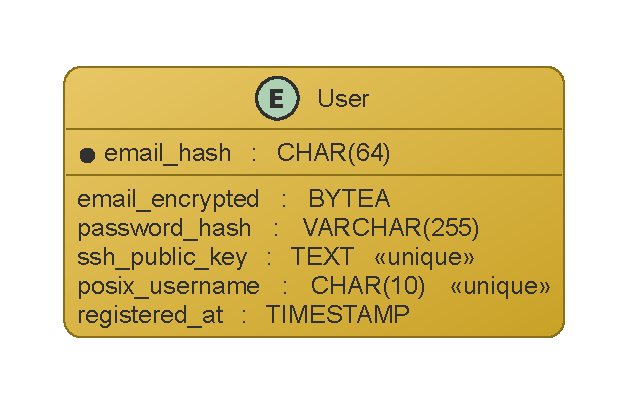
\includegraphics[width=0.35\textwidth]{figures/06-data-er-database-vault.pdf}
    \caption{Entity-Relationship diagram of the user record in Database-Vault.}
    \label{fig:er-database-vault}
\end{figure}

The email is encrypted, recoverable only with the master key, while the password is never recoverable, since
it is stored only in hashed form, as an Argon2id digest. Theft of, or unauthorized access to, the
database is therefore not enough to read either of them.

When a new user registers, after revalidating the input, Database-Vault attempts
to save the data in an atomic transaction, rejecting the request if the email or the SSH key is already
registered, but without specifying which of the two is wrong.
If the save succeeds, it asks Storage-Service to create the user's POSIX space.
If Storage-Service fails, it deletes the record just created; otherwise it informs
Security-Switch that the registration succeeded.

At login, it recomputes the hash of the received password and compares it with the stored one, then responds to
Security-Switch.

A nonexistent email and a wrong password produce the same response: in this way,
whoever attempts to log in cannot use it to discover which emails are registered.
\autoref{chap:sicurezza}, however, explains how an external user can try to determine whether
an email is already registered in the system, and also how a malicious administrator can obtain a
user's access credentials.


\subsection{Storage-Service}

Storage-Service hosts the users' backup files.
It never processes content in plaintext because, by design, it is not able to. Indeed, it receives only
files that have been deduplicated, compressed, and encrypted client-side with Restic \cite{restic-github}.

At Database-Vault's request, it creates a dedicated POSIX user, with neither an interactive shell nor a traditional
home directory. Each user instead has a writable space in their own subdirectory inside a chroot.
The filesystem structure is shown in \autoref{fig:filesystem-storage}.

\begin{figure}[H]
    \centering
    \begin{minipage}{0.85\linewidth}
    \dirtree{%
    .1 /storage/\DTcomment{root of all registered users}.
    .2 user\textless{}xxxxxx\textgreater{}/\DTcomment{owner \texttt{root:root}, permissions 0711}.
    .3 data/\DTcomment{owner \texttt{user\textless{}xxxxxx\textgreater{}}, permissions 0700}.
    }
    \end{minipage}
    \caption{Storage-Service filesystem structure, from \texttt{creator.go} and \texttt{dirmaker.go}
    \cite{ramusb-code-posixuser-owners,ramusb-code-posixuser-modes}.}
    \label{fig:filesystem-storage}
\end{figure}

Access to Storage-Service can only take place via the Secure Shell File Transfer Protocol (SFTP) \cite{sftp-filexfer},
with the SSH public key sent by the user during registration. Therefore neither
username and password authentication nor any other form of Secure Shell access outside SFTP is permitted.

On every connection, a dedicated \texttt{AuthorizedKeysCommand} binary queries Database-Vault to
obtain the user's current public key.
Any error in that call denies the connection, according to the fail-secure principle \cite{owasp-fail-securely}.

\subsection{Network-Manager}

Network-Manager is the administrator of the network rules. It is responsible for defining, modifying, and deleting the
rules that allow a user of the private mesh network to reach the other members.

During registration, it creates a dedicated Headscale user and the pre-auth key with which the user's
device will join the network.

During login, it assigns the user's node the Access Control List (ACL) tag that enables twelve-hour
temporary access to Storage-Service.
A periodic process checks expiries and removes the tag from expired nodes.

\subsection{Certificate-Authority}

Certificate-Authority is the system's private CA, based on \texttt{smallstep/certificates}
\cite{smallstep-certificates-github}.

It issues, renews, and revokes the mTLS certificates of every internal service, which makes it a
particularly critical component of the system, as well as the only one reachable by all internal services:
a malicious actor who managed to compromise it could issue forged certificates
for any organization.

Each service obtains its first certificate by contacting the CA using a bootstrap token distributed
manually by an operator out-of-band. A detailed explanation can be found in \autoref{sec:pki}.


\subsection{Headscale}

Headscale is a self-hosted implementation of the Tailscale control server \cite{headscale-github}.

It acts as the coordinator of the private mesh network: on every connection attempt between two nodes,
it enforces the reachability rules decided by Network-Manager. It also distributes, through
MagicDNS, the hostnames with which nodes resolve one another, allowing the client to locate
Storage-Service without knowing its IP address.

It also validates the pre-auth key of a new device at the moment it joins the mesh.

Unlike every other internal component except Entry-Hub, Headscale does not reside in the
private network but is reachable by anyone on the internet. \autoref{sec:paradosso-coordinatore} explores the reasons in depth.

\subsection{Mosquitto}

Mosquitto is the MQTT broker to which every service, once a minute, publishes its own operational metrics.

It enforces an ACL under which each service can write to its own topic, without ever being able to read from it,
while Metrics-Collector can only read the entire \texttt{metrics/\#} space, without ever writing to it.

\subsection{Metrics-Collector}

Metrics-Collector is the component that receives, validates, and persists the operational metrics
published by every service.

It discards every received metric whose \texttt{service} field does not match the topic it arrives from, and
persists the accepted metrics as a hypertable in TimescaleDB \cite{timescaledb-github}, with a retention of
thirty days and compression after seven days.

\subsection{Grafana}

Grafana is the visualization platform with which an administrator consults the health status and the
performance of the system \cite{grafana-github}.

It reads from TimescaleDB directly, without going through Metrics-Collector.
The Grafana dashboard shows response times, throughput, and active connections.
\autoref{chap:osservabilita} covers this observability pipeline in detail.

\clearpage

\autoref{fig:architecture-container} summarizes the architecture just described together with the
communication protocols used.

\begin{figure}[H]
    \centering
    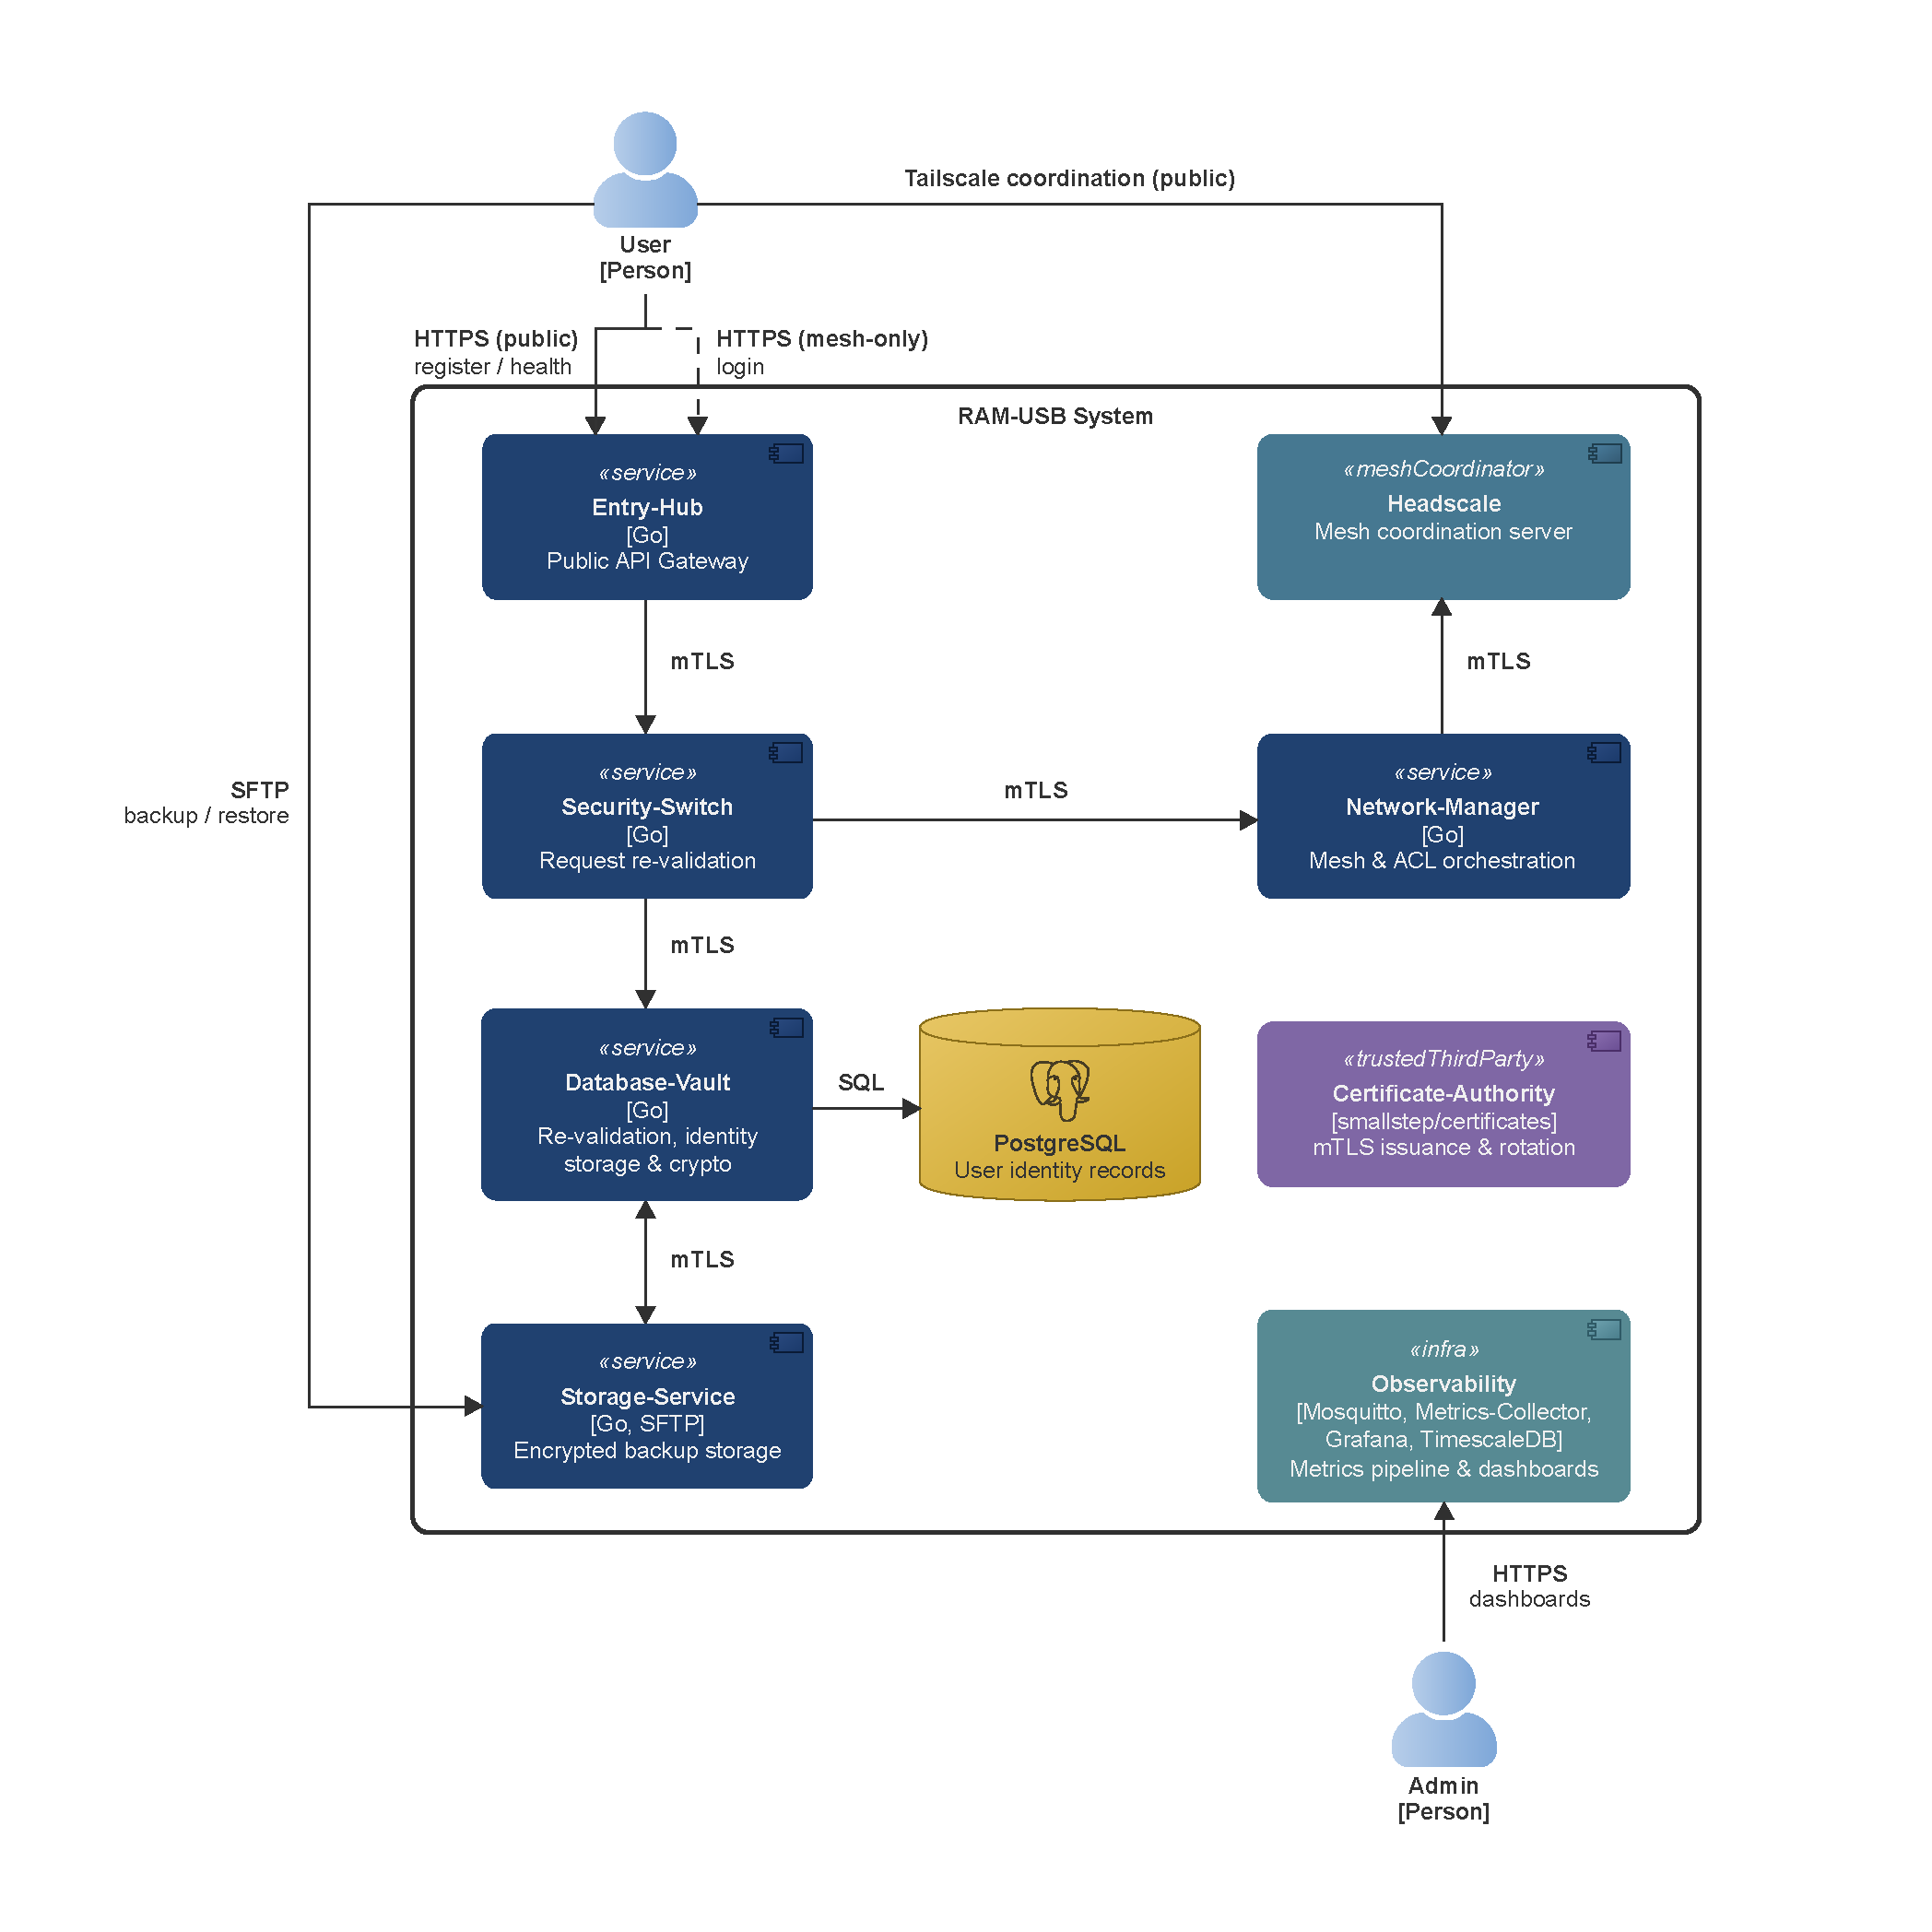
\includegraphics[width=0.8\textwidth]{figures/01-architecture-container.pdf}
    \caption{Container diagram of RAM-USB.}
    \label{fig:architecture-container}
\end{figure}

\section{Inter-service communication model}

Each service exposes its own HTTPS API built on Go's standard library, \texttt{net/http}.
Requests and responses are JSON bodies, and each endpoint is registered on a minimal router,
\texttt{http.ServeMux}. The minimum allowed TLS version is 1.3.

The endpoints listed here follow REST conventions \cite{fielding2000rest}.
\begin{itemize}
    \item \texttt{GET /api/health}, \texttt{POST /api/users} on Entry-Hub,
    \item \texttt{GET /internal/v1/public-key/\symbol{123}posix\_username\symbol{125}} on Database-Vault,
    \item \texttt{POST /internal/v1/posix-users} on Storage-Service, and
    \item \texttt{POST /internal/v1/mesh-users}, \texttt{POST /internal/v1/grants} on Network-Manager
\end{itemize}

\texttt{POST /api/login} is the only exception, because a successful login returns only the confirmation that
an action took place, with no identifier that a real \texttt{sessions} resource would require in order to
be read with GET or deleted with DELETE. The twelve-hour ACL token that the login grants remains
internal to Network-Manager and expires on its own.

The publication of metrics, moreover, is asynchronous: each service publishes its own messages on
a dedicated Message Queuing Telemetry Transport (MQTT) topic without any need to wait for a response.

This system structure comes at a significant cost: every registration and login passes through
four distinct processes, each with its own mTLS handshake and its own revalidation.
Latency is therefore much higher than in a monolithic system, and, should it ever need to be reduced, it cannot be
reduced by skipping one of the steps. Moreover, the service remains available to users only as long as
the seven components that take part in a request's path remain available, while the
observability chain can go down without the user noticing.

The two costs, however, are not of the same kind. Latency is inherent to the design and accepted together
with the architecture; availability, by contrast, is a deployment problem, and
\autoref{chap:deployment} discusses to what extent the underlying infrastructure is able to mitigate it.

\section{Trust zones and security boundaries}
\label{sec:trust-zones}

\autoref{fig:trust-zones} shows the reachability rules that Network-Manager applies to the mesh network.

The two outermost zones belong to the user, before and after authentication. A user who is registered but
not yet authenticated, and who therefore belongs to the \emph{Unauthenticated User Zone}, sees and can contact
only Entry-Hub. After login, the same node enters the \emph{Authenticated User Zone} and obtains
temporary reachability to Storage-Service.

Certificate-Authority reaches only the MQTT broker, but is reached by every other
internal component, to allow it to renew its own X.509 certificate.

The fourth zone, the \emph{Public Zone}, contains only Headscale, reachable from the public
network. \autoref{sec:paradosso-coordinatore} explains the reason in detail. However,
Network-Manager's calls to Headscale are still protected by mTLS authentication and
by the Headscale API key.

\begin{figure}[H]
    \centering
    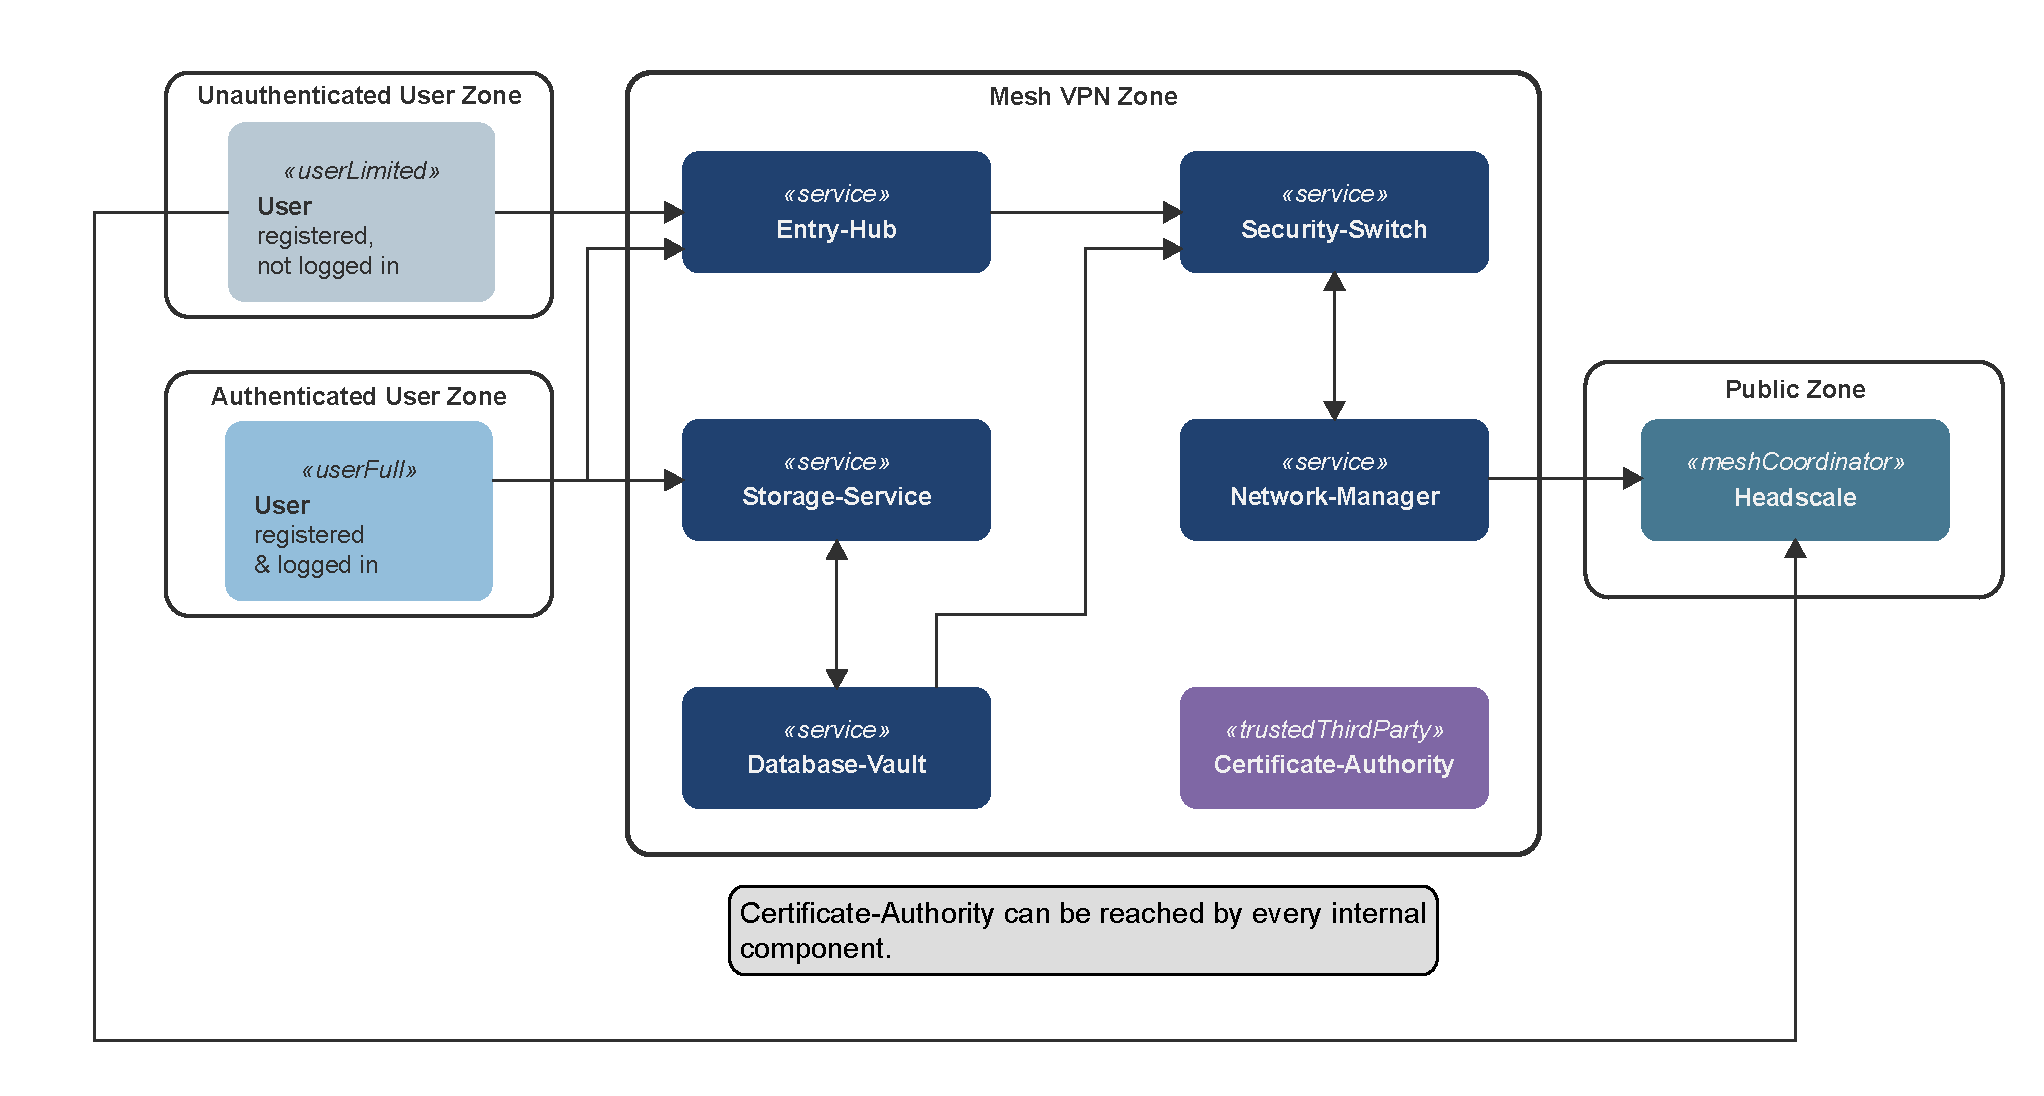
\includegraphics[width=0.8\textwidth]{figures/09-security-trust-zones.pdf}
    \caption{Trust zones and reachability on the mesh network.}
    \label{fig:trust-zones}
\end{figure}

\section{PKI and certificate management}
\label{sec:pki}

RAM-USB uses two certificate authorities, as illustrated in \autoref{fig:pki-hierarchy}.

Let's Encrypt, a public CA, signs only the certificate that Entry-Hub presents on its public
endpoints. This is because the certificate must be verifiable by an external client that does not yet have access
to the system's internal network. A certificate signed by RAM-USB's private Certificate-Authority would not
be trusted.

Every other communication instead uses the private Certificate-Authority, based on
\texttt{smallstep/\allowbreak certificates}.

Every private certificate follows the same bootstrap scheme: each service receives,
out-of-band and only once, a single-use bootstrap token, and presents it to Certificate-Authority
in exchange for its own initial certificate. Subsequent renewals present the mTLS certificate
already held. The token remains a throwaway secret and therefore does not need to be protected once
consumed.

A valid X.509 certificate only proves that Certificate-Authority approved that client, not that it is
the client expected for that connection. For this reason each service also verifies the
\texttt{organization} field of the certificate.

\begin{figure}[h]
    \centering
    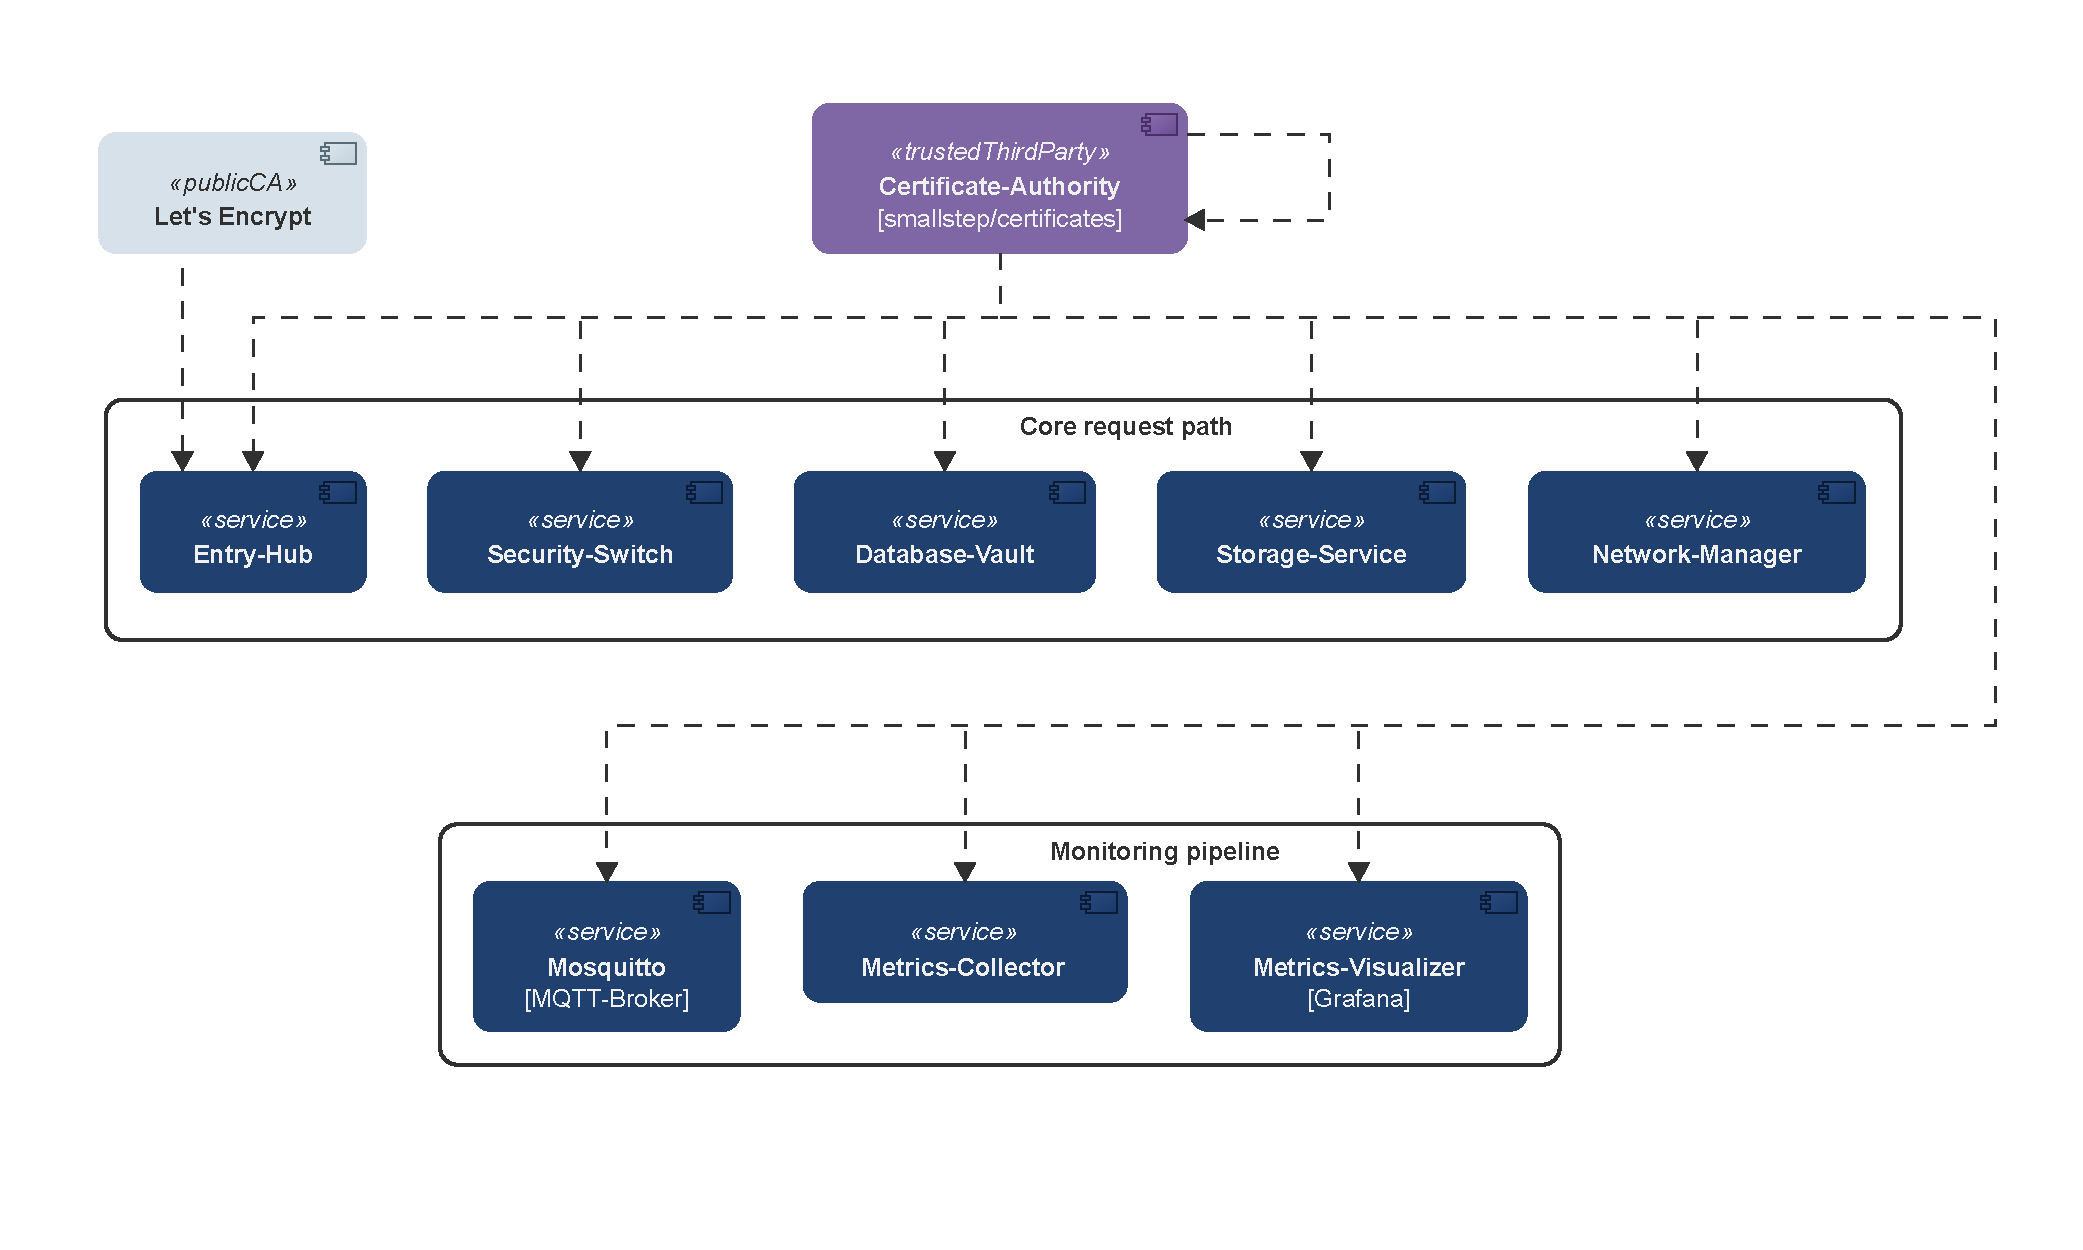
\includegraphics[width=\textwidth]{figures/08-security-pki-hierarchy.pdf}
    \caption{Hierarchy of the certificate authorities and signing relationships.}
    \label{fig:pki-hierarchy}
\end{figure}

